\documentclass[../TV&MS.tex]{subfiles}
\begin{document}
   
\section{Точечное оценивание}

\subsection{Эмпирическая функция распределения и её свойства}

\subsubsection{Вариационный ряд}

Как известно, функция распределения $F(x) = \Pro(X < x)$ однозначно определяет вероятностную меру.
Попробуем построить что-то похожее на функцию распределения.
Для этого мы возьмем нашу выборку $\Smpl = \left( X_1,\ldots X_n \right)$ и отсортируем по неубыванию.
Получим

\begin{Def}
    \mdef{Вариационный ряд} $\widetilde{\Smpl} = \left( X_{(1)},\ldots X_{(n)} \right)$"---~выборка, составленная из элементов исходной выборки, упорядоченных по неубыванию.
    Элементы вариационного ряда называются \mdef{порядковыми статистиками.}
\end{Def}

\begin{Note}
    Тут уже мы понимаем выборку в широком смысле, так как элементы вариационного ряда не являются независимыми и тем более не являются одинаково распределенными.
    Самое простое: если $X_{(1)} = 2$, то остальные элементы ряда заведомо не меньше $2$, то есть зависят от $X_{(1)}$. Дальше зависимость элементов показана аккуратно.
\end{Note} 

Теперь выведем функцию распределения $X_{(k)}$.
Наша цель~---~найти $F_{(k)}(x) = \Pro\left(X_{(k)} < x\right)$.
$X_{(k)} < x$ тогда и только тогда, когда хотя бы $k$ элементов выборки меньше $x$.
То есть возможны варианты для всех $i$ от $k$ до $n$, в каждом из которых ровно $i$ элемантов меньше $x$ и ровно $n-i$ элементов не меньше $x$.

\begin{equation}
    F_{(k)}(x) = \Pro\left( X_{(k)} < x \right) = 
    \sum\limits_{i=k}^{n} C_n^{i} \bigl( F(x) \bigr)^i \bigl( 1 - F(x) \bigr)^{n-i}
\end{equation} 

Напоминает схему испытаний Бернулли. Это она и есть.

\subsubsection{Эмпирическая ф.р.}

\begin{Def}\label{ms:ef:def:emp_func}
    \mdef{Эмпирическая (выборочная) функция распределения}
    \begin{equation}
        F_n(x) := \frac{1}{n}\sum\limits_{i=1}^{n} \Ind(X_{i} < x).
    \end{equation}   
\end{Def}

Выборочная функция распределения приближает истинную функцию распределения.
Смысл, в котором эмпирическая функция приближает истинную, раскрывается в пачке следующих теорем и утверждений.

\begin{St}
    \begin{equation}
        \Expec F_{n}(x) = F(x),
    \end{equation}
    где $F(x)$"---~истинная функция распределения.
\end{St} 

\begin{Proof}
    Зафиксируем $x$ и рассмотрим процесс генерации нашей выборки.
    Каждое испытание"---~генерация следующего значения из распределения.
    Будем считать, что $k$-е испытание успешное, если $X_{k} < x$.
    Тогда вероятность успеха в $k$-ом испытании
    $\Pro \left( X_k < x \right) = \Pro\left( X < x \right) = F(x)$,
    а сумма индикаторов $nF_n(x)$"---~число успехов в $n$ испытаниях.
    Поэтому мы можем записать, что $nF_n(x) \sim Bi(n, F(x))$.
    И из свойств биномиального распределения 
    $\Expec \bigl[ \cancel{n} F_n(x) \bigr] = \cancel{n}F(x) \Rightarrow
    \Expec F_n(x) = F(x)$.
\end{Proof} 

Теперь надо собрать волю в кулак и вспомнить усиленный закон больших чисел Колмогорова (УЗБЧ).
Он говорит, что для норсв с конечным МО $\frac{S_n}{n} \xrightarrow[]{\text{п.н.}} \Expec \xi$.
В нашем случае, он выглядит так:
\begin{equation}\label{msEmpirUzbch}
    F_n(x) \xrightarrow[]{\text{п.н.}} F(x).
\end{equation} 

А что это тут у нас тако-о-ое?
А это же функциональная последовательность!
А когда у нас функциональная последовательность куда-то сходится, что мы от неё хотим?
Пра-а-авильно, равномерной сходимости. Так вот есть такая

\begin{Th}[Гливенко]
    Эмпирическая функция распределения сходится к истинной равномерно с вероятностью 1.
    \begin{equation}
        \Pro \left( \lim\limits_{n \rightarrow \infty} \sup_{x} \bigl| F_n(x) - F(x) \bigr| = 0 \right) = 1.
    \end{equation} 
\end{Th} 

\begin{Proof}
    Для простоты докажем для абсолютно непрерывного случая.
    Пусть наша выборка генерируется из распределения с ф.р. $F(x)$.
    Тогда зафиксируем число $m$, и для него найдем числа
    $-\infty = x_0 < x_1 <\ldots< x_{m-1} < x_m = \infty$,
    такие что $F(x_j) - F(x_{j-1}) = \frac{1}{m}, \quad j = \overline{1,m}$.
    Теперь $\forall x\ \exists j=\overline{1,m}$, такое что $x \in \left[ x_{j-1}, x_j \right]$. Тогда
    \begin{equation}\label{glivProof_1}
        F_n(x)-F(x) \leqslant F_n(x_j)-F(x_{j-1})=F_n(x_j)-F(x_j)+\frac{1}{m},
    \end{equation}
    \begin{equation}\label{glivProof_2}
        F_n(x)-F(x) \geqslant F_n(x_{j-1})-F(x_{j})=F_n(x_{j-1})-F(x_{j-1})-\frac{1}{m}.
    \end{equation}
    Комбинируя \eqref{glivProof_1} и $\eqref{glivProof_2}$ и ещё там всякие модули, супремумы, получаем
    \begin{equation}
        \sup_x \bigl| F_n(x) - F(x) \bigr| \leqslant
        \max_{j \in \left\{ 1,\ldots m \right\}} 
        \bigl|F_n(x_j) - F(x_j) \bigr| + \frac{1}{m}
    \end{equation} 
    Теперь в силу~\eqref{msEmpirUzbch} 
    $\max\limits_{j \in \left\{ 1,\ldots m \right\}} \bigl|F_n(x_j) - F(x_j) \bigr|
    \xrightarrow{\text{п.н.}} 0$, поэтому $\forall m\ \exists N$,
    такой что $\forall n \geqslant N \quad \sup\limits_x \bigl| F_n(x) - F(x) \bigr| \leqslant \dfrac{1}{m} + \epsilon$.
    Наконец, полагая $m \rightarrow \infty$ и $\epsilon \rightarrow 0$,
    получаем утверждение теоремы.
\end{Proof} 

\begin{figure}
    \centering
    \begin{tikzpicture}
        \begin{axis}[
                area legend,
                xmin=-3,
                xmax=3,
                legend pos = outer north east,
                legend style = {fill=none}
            ]
            \addplot[
                line legend,
                const plot mark right,
                mark=o,
                blue
            ] table {data/ms_emp_func_sample.dat};
            \addlegendentry{Выборочная ф.р.}
            \addplot[
                line legend,
                mark=none,
                red,
                smooth
            ] table {data/ms_normal_distr_func.dat};
            \addlegendentry{Истинная ф.р.}
            \addplot[
                const plot mark right,
                green,
                name path = upper 
                ] table {data/ms_sample_upper.dat};
            \addplot[
                const plot mark right,
                green,
                name path = lower
                ] table {data/ms_sample_lower.dat};
            \addplot [green!20] fill between [
                    of = lower and upper,
                    soft clip = {domain = -4:4}
                ];
            \addlegendentry{См. зам. к~т.~\ref{ms:ef:th:kolmogorov}}
        \end{axis} 
    \end{tikzpicture} 
    \caption{Эмпирическая и истинная функции распределения.
    В качестве примера взята выборка размера $25$ из стандартного нормального распределения.}
    \label{ms:ef:fig:sample}
\end{figure}

Хорошо. Вот мы выяснили, что все хорошо и выборочная ф.р. благополучно сходится к теоретической.
Но сразу встает вопрос, а вот какой размер выборки мы можем считать достаточным?
Иными словами, нам интересна не только сам факт сходимости, но и скорость сходимости эмпирической ф.р. к теоретической.
А для этого на понадобится вот этот~\eqref{fXiOfXi} факт.
Обозначим $D_n = \sup\limits_x \bigl| F_n(x) - F(x) \bigr|$

\begin{Th}[Колмогорова]\label{ms:ef:th:kolmogorov}
    \[
        \Pro\left(\sqrt{n}D_n<x\right)=K_n(x)\quad\forall\ \text{ф.р.}\ F.
    \]
    \[
        \lim\limits_{n \rightarrow \infty} K_n(x) = K(x) = 
        \sum\limits_{k=-\infty}^{\infty} (-1)^{k} e^{-2k^2x^2} \Ind(x \ge 0)
    .\] 
\end{Th} 

\begin{Proof}
    Докажем только первую часть теоремы, а именно, что распределение $D_n$ не зависит от теоретической функции распределения.
    На $\sqrt{n}$ мы без зазрения совести забиваем, потому что он влияет только на вид распределения, но не на зависимость или независимость от $F$.
\begin{multline}
    \Pro \left( D_n < x \right) = 
    \Pro \left( \sup\limits_y \bigl| F_n(y) - F(y) \bigr| < x \right) = \\
    = \left\{ \text{\parbox{4cm}{\footnotesize
            Считаем, что $F(x)$ непрерывна и строго монотонна и полагаем
            $y = F^{-1}(z)$
    }} \right\}
    = \Pro \left( \sup_{0 \le z \le 1} \Bigl\lvert F_n\bigl(F^{-1}(z)\bigr) -
        F\bigl(F^{-1}(x)\bigr)\Bigr\rvert < z \right) = \\
    = \Pro \left( \sup_{0 \le z \le 1} \Bigl\lvert F_n\bigl(F^{-1}(z)\bigr) -
        z \Bigr\rvert < z \right)
    =  \Pro \left( \sup_{0 \le z \le 1} \left\lvert \frac{1}{n}
        \sum\limits_{i=1}^{n} \Ind \bigl(X_i < F^{-1}(z)\bigr) -z \right\rvert
        < z \right) = \\
    = \Pro \left( \sup_{0 \le z \le 1} \left\lvert \frac{1}{n}
        \sum\limits_{i=1}^{n} \Ind \bigl(F(X_i) < z\bigr) - z \right\rvert
        < z \right)
    = \left\{ \parbox{3.1cm}{$U_i := F(X_i),\\
        U_i \sim U[0,1]$~\eqref{fXiOfXi}} \right\} = \\
    = \Pro \left( \sup_{0 \le z \le 1} \left\lvert \frac{1}{n}
        \sum\limits_{i=1}^{n} \Ind \bigl(U_i < z\bigr) - z \right\rvert
        < z \right)
\end{multline} 
\end{Proof}

\begin{Note}
    Какой первый вопрос, который возникает у каждого трушного прикладного математика, когда он видит подобную теорему?
    Конечно! Всем интересно, чему равна бесконечность.
    Иными словами, при каком размере выборки мы можем благополучно использовать $K(x)$ вместо унылых $K_n(x)$?
    Так вот для этой теоремы считается, что $\infty = 20$.
    Как обычно пользуются этой теоремой? Как-то так:
    \begin{enumerate}
        \item Определение границ, в которых с заданной вероятностью находится теоретическая функция распределения.
            Давайте для нашей выборки~(рис.~\ref{ms:ef:fig:sample}) построим границы, в которой с вероятностью $0,8$ находится теоретическая ф.р.
            $0,8$-квантиль распределения Колмогорова примерно равна $1,07$.
            То есть в нашем случае 
            $0,8=\Pro\left(\sqrt{25}D_{25}<1,07\right)=
            \Pro\left(D_{25} < 0,214 \right)$.
            И вот таким вот макаром мы получили зелёного крокодила на рис.~\ref{ms:ef:fig:sample}.
        \item Проверка гипотез. Эту тему мы будем мусолить позже, пока кратко.
            Вот кинули в нас выборкой, и сказали: <<а ну ка отвечай, может это
            быть выборкой из такого-то распределения с такими-то параметрами?>>
            Тут можно построить выборочную функцию распределения и посчитать, насколько максимум выборочная ф.р. 
            отличается от теоретической, которую мы хотим проверить, и посмотреть вероятность, 
            с которой можно встретить такое отклонение.
            Если вероятность маленькая, то, скорее всего, нам присунули 
            какую-то левую выборку, а если большая, то надо кастовать 
            магическое заклинание <<данные не противоречат>>, 
            о котором будет позже.
    \end{enumerate} 
\end{Note}

\begin{figure}
    \centering
    \begin{minipage}[t]{.5\textwidth}
        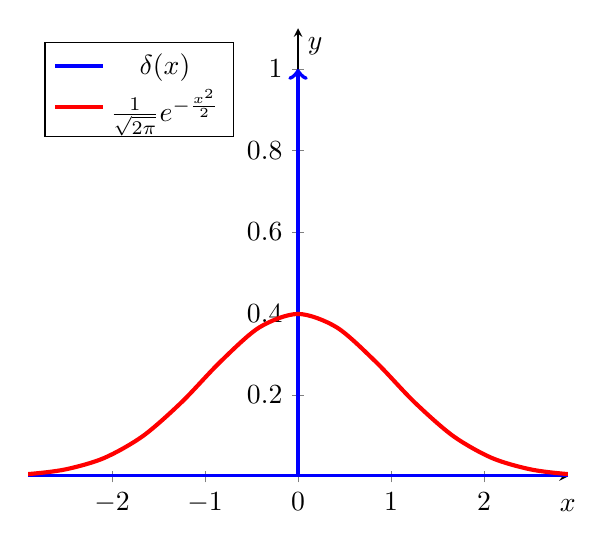
\begin{tikzpicture}
            \begin{axis}[
                xmin = -2.9,
                xmax = 2.9,
                axis x line = bottom,
                axis y line = middle,
                ymax = 1.1,
                xlabel = $x$,
                ylabel = $y$,
                every axis x label/.style = {
                    at = {(ticklabel cs:1)}, anchor = south
                },
                legend style = {fill = none, legend pos = north west},
            ]
            \draw [blue, line width = 1.5pt, ->] (axis cs: {0},{0}) -- (axis cs:{0},{1});
            \addplot[
                mark = none,
                blue,
                line width = 1.5pt
            ] coordinates {
                (-2.9, 0)
                (2.9, 0)
            };
            \addlegendentry{$\delta(x)$}
            \addplot[
                mark = none,
                smooth,
                red,
                line width = 1.5pt,
            ] expression {1/sqrt(2*pi) * e^(-x^2/2)};
            \addlegendentry{$\frac{1}{\sqrt{2\pi}}e^{-\frac{x^2}{2}}$}
            \end{axis} 
        \end{tikzpicture} 
        \caption{Различные варианты ядра.}
        \label{ms:ef:fig:kernels}
    \end{minipage}%
    \hfill
    \begin{minipage}[t]{.5\textwidth}
        \begin{tikzpicture}
            \begin{axis}[
                xmin = -2.9,
                xmax = 2.9,
                axis x line = bottom,
                axis y line = middle,
                ymax = 1.1,
                xlabel = $x$,
                ylabel = $y$,
                every axis x label/.style = {
                    at = {(ticklabel cs:1)}, anchor = south
                },
                legend style = {fill = none, legend pos = north west},
            ]
            \addplot[
                mark = o,
                blue,
                line width = 1.5pt
            ] coordinates {
                (-3, 0)
                (0, 0)
            };
            \addlegendentry{$\Ind(x < 0)$}
            \addplot[
                mark = none,
                smooth,
                red,
                line width = 1.5pt,
            ] table {data/ms_normal_distr_func.dat};
            \addlegendentry{$\Phi(x)$}
            \addplot[
                mark = *,
                blue,
                line width = 1.5pt
            ] coordinates {
                (0, 1)
                (3, 1)
            };
            \end{axis} 
        \end{tikzpicture} 
        \caption{Соответствующие функции распределения.}
        \label{ms:ef:fig:kerDistrFuncs}
    \end{minipage} 
\end{figure}

\subsubsection{Ядерные оценки}

Эмпирическая функция распределения великолепна и достойна всяческого восхищения.
Но у неё есть один недостаток: она разрывна и не строго монотонна, а мы любим, когда все хорошо, монотонно и непрерывно. 
Что делать?
Введем функцию $k(x)$, которую заставим обладать следующими свойствами:
\begin{equation}\label{ms:ef:eq:prop_1}
    k(x) \ge 0 \quad \forall x \in \Real,
\end{equation}
\begin{equation}\label{ms:ef:eq:prop_2}
    \int\limits_{-\infty}^{\infty} k(x)\,dx = 1,
\end{equation}
\begin{equation}\label{ms:ef:eq:prop_3}
    \int\limits_{-\infty}^{\infty} xk(x)\,dx = 0,
\end{equation} 
\begin{equation}\label{ms:ef:eq:prop_4}
    \int\limits_{-\infty}^{\infty} x^2k(x)\,dx = 1
.\end{equation} 

Что сейчас только что произошло? 
Свойствами~\eqref{ms:ef:eq:prop_1} и~\eqref{ms:ef:eq:prop_2}
мы сказали, что хотим корректную функцию плотности,
а свойствами~\eqref{ms:ef:eq:prop_3} и~\eqref{ms:ef:eq:prop_4}
мы пронормировали это безобразие на нулевое матожидание и единичную дисперсию.
Теперь введем для нашего ядра функцию распределения:

\begin{equation}
    K(x) := \int\limits_{-\infty}^{x} k(x)\,d~
.\end{equation}
И в выражение для выборочной ф.р. подставим в общем случае ф.р. ядра:

\begin{equation}
    F_{n}^{K}(x) = \frac{1}{n}\sum\limits_{i=1}^{n} \frac{1}{h_i} K\left(\frac{x - X_{i}}{h_i}\right)
,\end{equation} 
где $X_i$ \textit{символизирует} матожидание, то есть, что мы пляшем вокруг
конкретного элемента выборки, а $h_i$ позволяет управлять крутизной
функции распределения и \textit{символизирует} дисперсию.
Теперь, если мы в качестве функции ядра выберем $\delta$-функцию
(с оговоркой, что говорить про дисперсию будет совсем некорректно), 
то мы получим классическую выборочную функцию распределения,
как в определении~\ref{ms:ef:def:emp_func}.
Но поскольку самое пацанское распределение~---~это нормальное распределение,
то в качестве ядра можно выбрать и $k(x) = (2\pi)^{-1\!/2}e^{-x^2\!/2}$, тогда получим
оценку теоретической функции распределения, как на графике на рис~\ref{ms:ef:fig:compKer}. 

\begin{figure}
    \centering
    \begin{tikzpicture}
        \begin{axis}[
                xmin = -3.9,
                xmax = 3.9,
                axis x line = bottom,
                axis y line = middle,
                ymax = 1.1,
                xlabel = $x$,
                ylabel = $y$,
                every axis x label/.style = {
                    at = {(ticklabel cs:1)}, anchor = south
                },
                legend style = {fill = none, legend pos = outer north east},
            ]
            \addplot[
                const plot mark right,
                blue,
                line width = 1.5pt,
                mark = o,
            ] table {data/ms_ef_ker_ind.dat};
            \addlegendentry{Ф.р. для $k(x) = \delta(x)$}
            \addplot[
                smooth,
                red,
                line width = 1.5pt,
                mark = none,
            ] table {data/ms_ef_ker_ker.dat};
            \addlegendentry{Ф.р. для $k(x)=\frac{1}{\sqrt{2\pi}}e^{-x^2\!/2}$}
            \addplot[
                smooth,
                green,
                line width = 1.5pt,
                trig format = rad,
            ] expression {0.5 + 1 / pi * atan(x)};
            \addlegendentry{Теор. ф.р. $\frac{1}{2}+\frac{1}{\pi}\arctg{(x)}$}
        \end{axis} 
    \end{tikzpicture} 
    \caption{Приближение теоретической функции рспределения выборочной и
        ядерная оценка с использованием функции плотности нормального распределения.}   
    \label{ms:ef:fig:compKer}
\end{figure} 

\newpage

\end{document}
